\graphicspath{{chapters/01/images/}}
\chapter{Introduction}

\section{Bioinformatics}
Bioinformatics can be defined as the development of new algorithms and statistical methods that allow to establish relations between members of huge sets of data.
It can also be described as the analysis and interpretation of different data types including nucleotide and amino acid sequences, protein domains and protein structures.
The development and implementation of these programs allow efficient access and management of different types of information.

	\subsection{The human genome}
	The human genome contains around $3.2$ billion base pairs.
	About $80\%$ of it is associated with a biochemical function.
	Of particular interest is non-coding DNA, which doesn't code for proteins but is mainly involved in:

	\begin{multicols}{3}
		\begin{itemize}
			\item Protection of the genome.
			\item Gene switches.
			\item Gene expression regulation.
			\item Transcription factor binding sites.
			\item Operators.
			\item Enhancers.
			\item Promoters.
			\item Silencers.
		\end{itemize}
	\end{multicols}

\section{Involvement of computer science}
Computer science plays a fundamental part in bioinformatics, providing the algorithms necessary to exploit data collected in experiment to reach a significant conclusion.

	\subsection{Databases}
	Databases or data banks are collections of correlated data utilized to represent a portion of the real world.
	They are structured in a way to allow data organization and management in terms of:

	\begin{multicols}{4}
		\begin{itemize}
			\item Insertion.
			\item Update.
			\item Search.
			\item Deletion.
		\end{itemize}
	\end{multicols}

	\subsection{Program}
	A program codifies an algorithm into a programming language.
	It is used to test and realize a proposed solution.
	Computer science can be defined as the science of the automatic elaboration of information, with algorithms as its central focus.

	\subsection{Algorithm}
	Algorithms (from the name of the Persian mathematician \textit{Muhammad ibn Musa al-Khwarizmi}) can be defined as a system of well-defined rules and procedures that lead to the solution of a problem with a finite number of steps.
	They can be described in pseudo-code.

		\subsubsection{Substring search algorithm}
		A substring search algorithm is an algorithm that searches the occurrence of a string in another, allowing to understand if the former is contained in the latter.
		A na\"ive implementation is described in figure \ref{fig:substring-search-naive}.

		\begin{figure}[H]
			\centering
			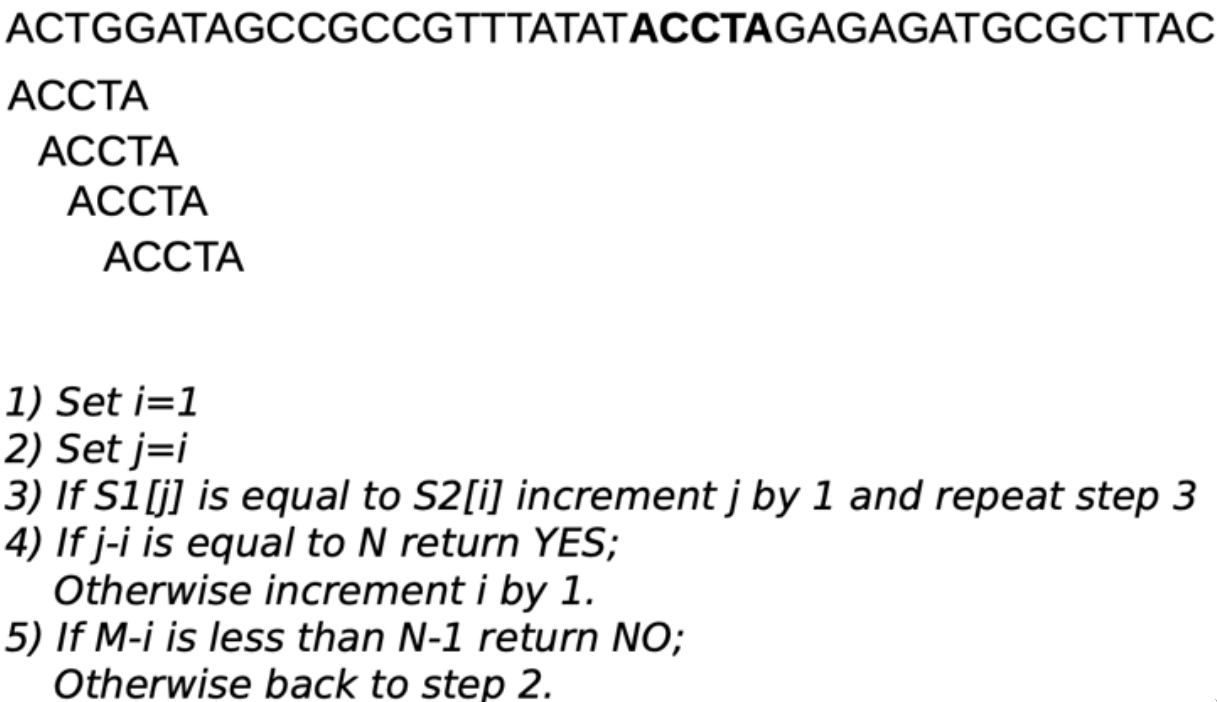
\includegraphics[width=0.6\textwidth]{substring-search}
			\caption{Na\"ive implementation of a substring search algorithm}
			\label{fig:substring-search-naive}
		\end{figure}
